\documentclass[11pt]{report}
\usepackage[margin=1in]{geometry}
\usepackage{titlesec}
\usepackage{graphicx}
\usepackage{parskip}
\usepackage{glossaries}
\usepackage{datetime}

\titleformat{\chapter}{\Large\bfseries}{}{0pt}{\huge}
\titlespacing\chapter{0pt}{*1}{*1}
\titlespacing\section{0pt}{*0}{-\parskip}
\titlespacing\subsection{0pt}{*0}{-\parskip}
\titlespacing\paragraph{0pt}{*0}{*3}

\newcommand*{\TitleFont}{
      \usefont{\encodingdefault}{\rmdefault}{b}{n}
      \fontsize{24}{36}
      \selectfont
}
\newcommand{\thickline}{\rule{\textwidth}{1.6pt}}
\newcommand{\thinline}{\rule{\textwidth}{0.4pt}}
\newcommand{\novspace}{\vspace*{-\baselineskip}\vspace*{4pt}}
\renewcommand{\dateseparator}{-}
\let\oldtitle\title
\renewcommand{\title}[1]{\oldtitle{\thickline \\ \novspace \thinline \\ \TitleFont {#1} \thinline \\ \novspace \thickline}}
\newcommand{\tableoffiguresandtables}{\listoffigures\begingroup\let\clearpage\relax\listoftables\endgroup}

\author{
	Evan Milton \\
	Computer and Electronics Engineering \\
	University of Nebraska at Lincoln - Omaha Campus \\
	Electronics Engineering
		\and
	Josh DeWitt \\
	Computer and Electronics Engineering \\
	University of Nebraska at Lincoln - Omaha Campus \\
	Computer Engineering and Mathematics, minor in Computer Science
		\and
	Chad Staley \\
	Computer and Electronics Engineering \\
	University of Nebraska at Lincoln - Omaha Campus \\
	Electronics Engineering
		\and
	James Gehringer \\
	Computer and Electronics Engineering \\
	University of Nebraska at Lincoln - Omaha Campus \\
	Computer Engineering, minor in Computer Science
}
\date{\yyyymmdddate\today}

\newacronym{2d}{2-D}{Two-Dimensional}
\newacronym{3d}{3-D}{Three-Dimensional}
\newacronym{aon}{AON}{Activity On Node}
\newacronym{arm}{ARM}{Advanced RISC Machines}
\newacronym{bom}{BOM}{Bill of Materials}
\newacronym{cad}{CAD}{Computer-Aided Design}
\newacronym{ceen}{CEEN}{Computer and Electronics Engineering}
\newacronym{cnc}{CNC}{Computer Numerical Control}
\newacronym{cpu}{CPU}{Central Processing Unit}
\newacronym{dmm}{DMM}{Digital Multi-Meter}
\newacronym{drc}{DRC}{Design Rules Check}
\newacronym{dvi}{DVI}{Digital Visual Interface}
\newacronym{eco}{ECO}{Engineering Change Order}
\newacronym{ecr}{ECR}{Engineering Change Request}
\newacronym{gpio}{GPIO}{General Purpose Input/Output}
\newacronym{led}{LED}{Light Emitting Diode}
\newacronym{lrc}{LRC}{Linear Responsibility Chart}
\newacronym{pcb}{PCB}{Printed Circuit Board}
\newacronym{pi}{Pi}{Raspberry Pi}
\newacronym{pcsc}{PCSC}{Project Common Success Criteria}
\newacronym{pssc}{PSSC}{Project Specific Success Criteria}
\newacronym{tcpip}{TCP/IP}{Transmission Control Protocol/Internet Protocol}
\newacronym{ti}{TI}{Texas Instruments}
\newacronym{wbs}{WBS}{Work Breakdown Structure}
\newacronym{xp}{XP}{Extreme Programming}

\date{2013-12-12}
\titleandsubtitle{CNC Interface \\ Team 3 - Project Proposal}{A planning document for a Senior Thesis Project submitted to the faculty of \\ Computer and Electronics Engineering \\ University of Nebraska-Lincoln \\ College of Engineering \\ Peter Kiewit Institute}

\begin{document}
{\centering\chapter{Team 3 Objective Tree and PSSC Update}}

\section{Objective Tree}
Figure ~\ref{fig:o-tree} outlines the requirements for having a functioning \gls{cnc} interface for this Senior Thesis Project.
Safety is the most important objective in this project since the \gls{cnc} interface will control moving components, although these moving components are outside the scope of this report.
Next most important is the \gls{cnc} functionality, otherwise the interface would not be able to control any \gls{cnc}.
Speed and accuracy is rated next most important to ensure the movements coordinated by the interface are as closed to the desired as possible.
The \gls{cnc} control is required to allow G-Code to be uploaded to the system and allow system monitoring.
A variable power input is desired so that users may purchase a power supply that fits their motors' needs, ensuring that a properly priced power supply is bought for the system.

\begin{figure}[H]
\centering
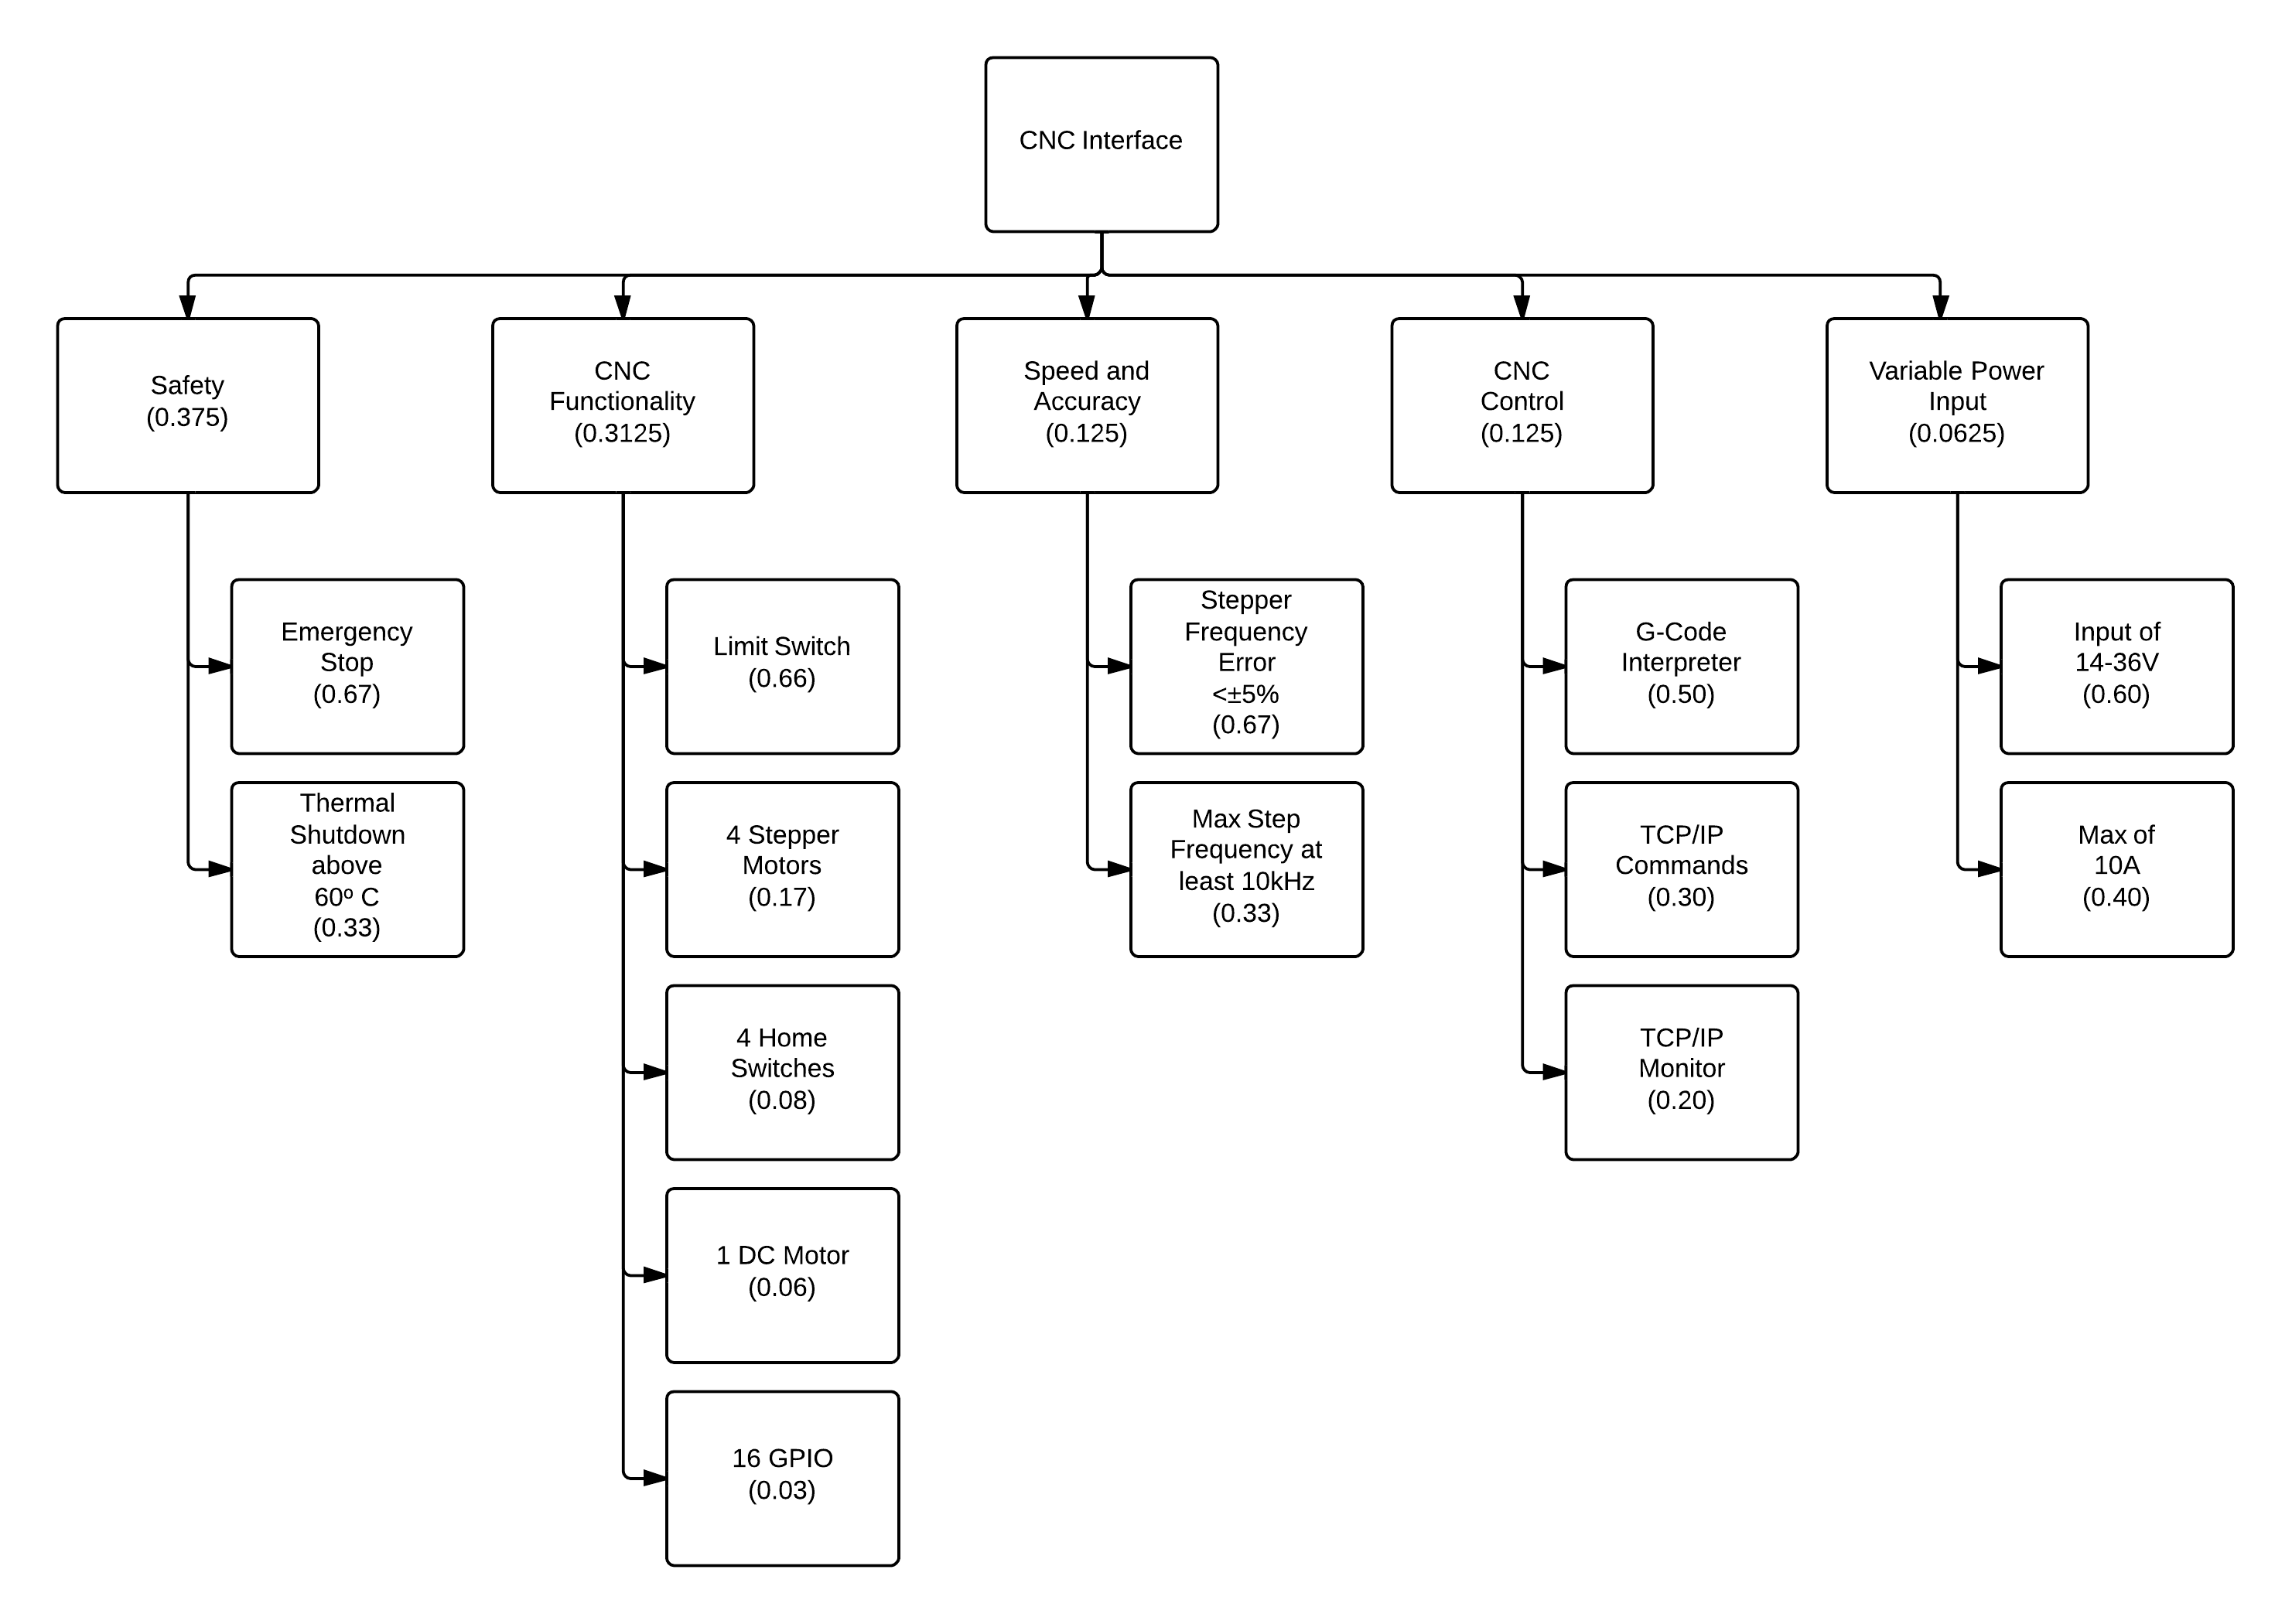
\includegraphics[width=1.0\textwidth]{otree.png}
\caption{Objective Tree}
\label{fig:o-tree}
\end{figure}

\section{Success Criteria}
The project's success will be determined by whether or not the 10 engineering requirements, consisting of 5 \gls{pcsc} and 5 \gls{pssc}, are met. 

\subsection{Five Project Common Success Criteria}
\begin{enumerate}
	\item Create a complete \gls{bom} and order/sample all parts needed for the design.
	\item Develop complete, accurate, readable schematic of the design, complete with interface loading analysis and interface timing analysis. 
	\item Complete a layout and etch a \gls{pcb}.
	\item Populate and debug the design on a custom \gls{pcb}.
	\item Professionally package the finished product and demonstrate its functionality.
\end{enumerate}

\subsection{Five Project Specific Success Criteria}
\begin{enumerate}
	\item The system will drive at least 4 stepper motors, 1 DC motor, and 16 General Purpose Outputs.
The system will receive inputs from at least 1 emergency stop switch and 4 stepper motor home inputs.
	\item The system will Receive G-code through \gls{tcpip}.
The system’s software will be developed using IEEE Std 830-1998 Recommended Practice for Software Requirements Specifications.
	\item The step frequency range will be at a minimum of 10kHz.
For any chosen frequency in range, the actual step frequency will be within 5\% of the desired frequency.
	\item The system power supply will accept between 14V and 36V and draw a maximum of 10A, including current required for the motors. 
	\item The system will stop all motors and shutdown all microcontrollers if the main microcontroller temperature reaches $60^{\circ}C$.
\end{enumerate}

\newpage
\section{Approval}
By signing below, I hereby approve of the objectives and proposed \gls{pssc}s for this project. 

\begin{tabular}{ca{8cm}ca{4cm}c}\signature{Evan Milton}\signature{Josh DeWitt}\signature{Chad Staley}\signature{James Gehringer}\signature{Herb Detloff}\end{tabular}
\end{document}
